\section{匹配与因子分解}

\subsection{匹配}
\subsubsection{图的匹配相关概念}
\begin{enumerate}
	\item 给定图$G=(V,E)$.设$M$是$E$的不包含环的子集,它的任意两条边在$G$中均不相邻,则称$M$是$G$的\colorbox{yellow}{\textcolor{red}{匹配}}.
	\item 如果$M$是图$G$的包含边数最多的
	匹配,称$M$是$G$的一个\colorbox{yellow}{\textcolor{red}{最大匹配}}. 特别是,若最大匹配
	饱和了$G$的所有顶点,称它为$G$的一个\colorbox{yellow}{\textcolor{red}{完美匹配}}.
	\begin{figure}[H]
		\small
		\centering 
		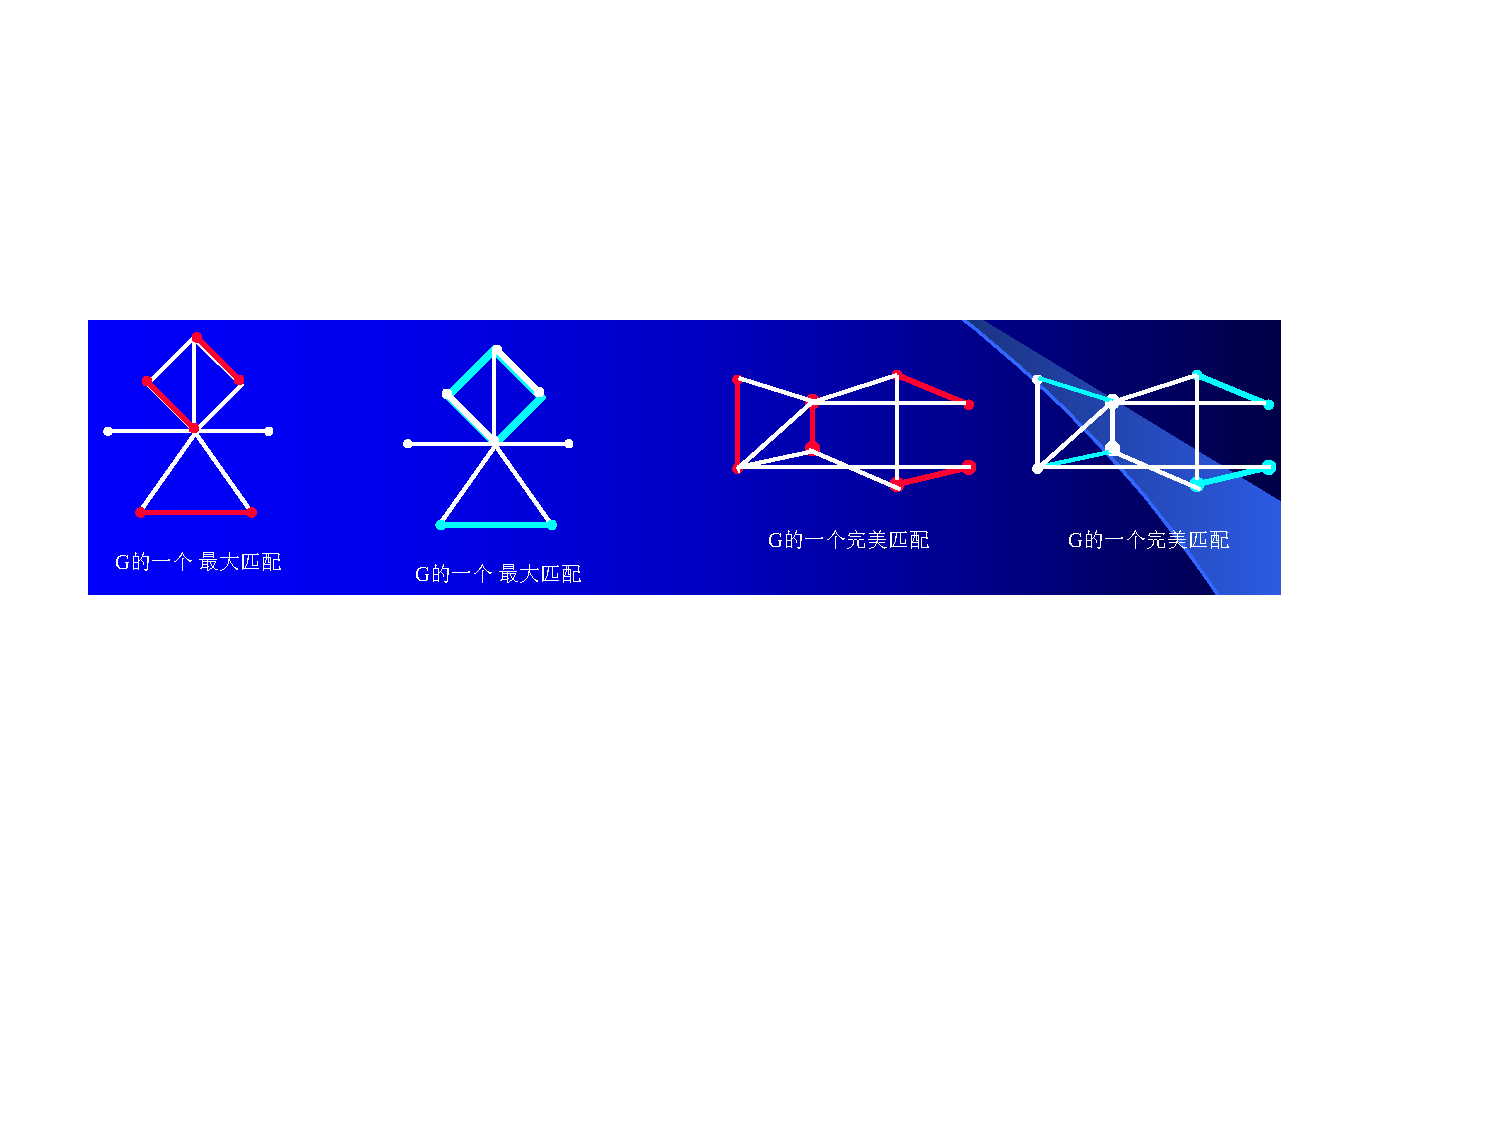
\includegraphics[scale=0.65]{image/CH5_pipei.pdf}  
		%\caption{信息包结构} 
		\label{fikgkjjj1KKik}  
	\end{figure}
	\begin{note}
		\begin{enumerate}
			\item 一个图G不一定存在完美匹配.
			\item 一个图G的完美匹配若存在,不一定唯一.
			\item 一个图G的最大匹配不一定唯一.
			\item \textcolor{red}{完美匹配一定是最大匹配,最大匹配不一定是完美匹配}.
		\end{enumerate}
	\end{note}
	\item 如果$M$是图$G$的匹配,$G$中一条由$M$中的边和非$M$中的边交错形成的路,称为G中的一条\colorbox{yellow}{\textcolor{red}{$M$
	交错路}}.特别地,若$M$交错路的起点与终点是\textcolor{red}{$M$非饱和
	点},称这种$M$交错路为\colorbox{yellow}{\textcolor{red}{$M$可扩路}}.
		\begin{note}
			如果$G$中顶点$v$是$G$的匹配 $M$中某条边的端点,称它
			为\textcolor{red}{$M$饱和点},否则为\textcolor{red}{$M$非饱和点}.
		\end{note}
\end{enumerate}
\subsubsection{贝尔热定理}
\begin{theorem}[贝尔热,1957]
	\colorbox{yellow}{$G$的匹配$M$是最大匹配,当且仅当$G$不包含$M$可扩路}.
\end{theorem}




\subsection{偶图的匹配和覆盖}
\subsubsection{偶图的匹配}

\begin{theorem}[Hall,1935]
	设$G=(X, Y)$是偶图,则$G$存在饱和$X$每个
	顶点的匹配的充要条件是:
	\[
	\colorbox{yellow}{$|N(S)|\geq |S|,\mbox{对}\forall S \subseteq X \mbox{成立}$}.
	\]
\end{theorem}
\begin{note}
	\textcolor{red}{$N(S): S$的\colorbox{yellow}{邻集}$-$与$S$的顶点相邻的所有顶点的集}.匈牙利算法的基础.
\end{note}

\begin{example}[常考大题应用题]
	内容...
\end{example}
\begin{corollary}
	若$G$是$k (k>0)$正则偶图,则$G$存在完美匹配.
\end{corollary}

\begin{note}
	\begin{enumerate}
		\item 每个\textcolor{red}{$k$方体}都有完美匹配($k\geq 2$).
		\item 树至多存在\textcolor{red}{一个}完美匹配.
		\item \colorbox{yellow}{$K_{2n}$}不同完美匹配个数为\colorbox{yellow}{$(2n-1)!!$}.
		\item \colorbox{yellow}{$K_{n,n}$} 不同完美匹配个数为\colorbox{yellow}{$n!$}.
		
	\end{enumerate}
\end{note}



\subsubsection{点覆盖与哥尼定理}
\begin{definition}
	$G$的一个\colorbox{yellow}{\textcolor{red}{点覆盖}}是指$V(G)$的一个\textcolor{red}{顶点子集$K$},使得$G$的每条边都至少有一个有一个端点在$K$之中. $G$的一个包含点数最少的点覆盖称为$G$的\colorbox{yellow}{\textcolor{red}{最小点覆盖}},其包含的点数称为$G$的\textcolor{red}{覆盖数,记为$\alpha(G)$}.
\end{definition}

\begin{theorem}
	设$M$是$G$的匹配,$K$是$G$的覆盖,若	\colorbox{yellow}{$|M|=|K|$},则
	\textcolor{red}{$M$是最大匹配,而$G$是最小覆盖}.
\end{theorem}
\begin{proof}
	$K$至少包含$M$中每条边的一个端点,则$|M|\leq |K|\Rightarrow |M^{*} |\leq |K^{*}|\Rightarrow |M|\leq |M^{*} \leq |K^{*}| \leq |K|$. 又因为$|M|=|K|$,故$|M|=|M^{*} |, |K|=|K^{*}|$.
\end{proof}


\begin{theorem}[哥尼,1931]
	\colorbox{yellow}{在偶图中,最大匹配的边数等于最小覆盖的顶点数}.
\end{theorem}

\begin{note}
	 $K_{m,n}(m \leq n)$ 的最小覆盖包含的点数为 $\min\{m, n\}$.
\end{note}

\begin{example}
	矩阵的一行或一列称为矩阵的一条线。证明:布
	尔矩阵中,包含了所有“1”的线的最少数目,等于具有
	性质“任意两个1都不在同一条线上的1的最大数目”.
\end{example}
\begin{figure}[H]
	\small
	\centering 
	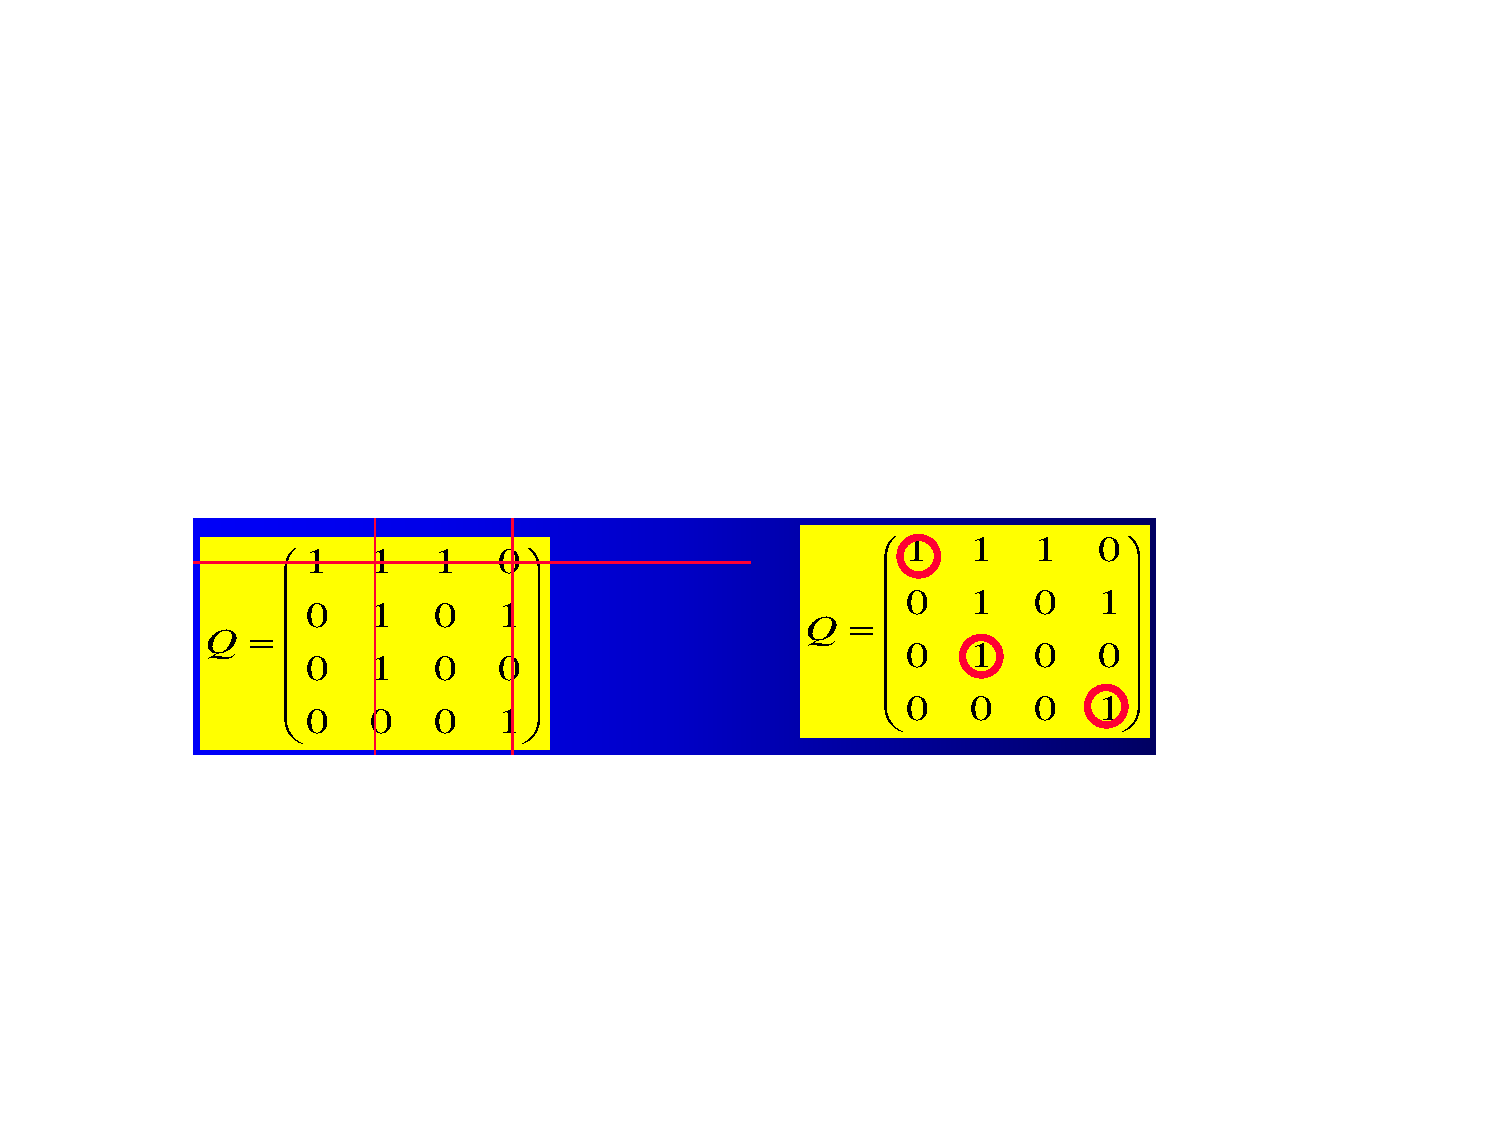
\includegraphics[scale=0.9]{image/CH5_233.pdf}  
	%\caption{信息包结构} 
	\label{fikgkjjj1KKk}  
\end{figure}
\begin{proof}
	设布尔阵是$n$行$m$列矩阵,把它模型为一个偶图
	如下:每行每列分别用一个点表示,$X$表示行点集合,$Y$
	表示列点集合,两点连线,当且仅当该行该列元为1.
	
	于是,包含了所有“1”的线的最少数目对应偶图中的
	最小点覆盖数。而具有性质“任意两个1都不在同一条
	线上的1的最大数目” 对应偶图的最大匹配包含的边数.
	
	由哥尼定理,命题得到证明。
\end{proof}






\subsection{托特定理与完美匹配}
\begin{theorem}[托特,1947]
	图$G$有完美匹配当且仅当对$V$
	的任意非空真子集$S$, 有
	\[
	\colorbox{yellow}{$o(G-S)\leq |S|$}.
	\]
\end{theorem}
\begin{note}
	\textcolor{red}{ $o(G-S)$表示奇分支数目}(奇分支表示顶点数为奇数).
\end{note}
\begin{example}
	证明:一棵树$G$有完美匹配当且仅当对所有顶点$v
	\in (G)$,有:$o(G-v)=1$.
\end{example}
\begin{proof}
\noindent 必要性:

一方面:若$G$有完美匹配,由托特定理:$o(G-v)\leq1$;另一方面:若树$G$有完美匹配,则显然$G$为偶阶树,于是$o(G-v)\geq1$; 所以:$o(G-v)=1$.

\noindent 充分性:

由于对任意点$v \in o(G-v)$, 有$o(G-v)=1$. 设$C_v$是$G-v$的奇分支,又设$G$中由$v$连到$G-v$的奇分支的
边为$vu$,显然,由$u$连到$G-u$的奇分支的边也是$uv$.令$M=\{e(v)$:它是由$v$连到$G-v$的奇分支的边,$v \in V(G) \}$则:$M$是$G$的完美匹配.
\end{proof}











\begin{corollary}[彼得森]
	\colorbox{yellow}{没有割边的3正则图存在完美匹配}.
\end{corollary}
\begin{note}
	有割边的 3 正则图不一定就没有完美匹配.
	
	彼得森图有完美匹配,3正则$H$图存在完美匹配.
\end{note}

\subsection{因子分解}
\subsubsection{1-因子分解}

\begin{definition}
	\begin{enumerate}
		\item 一个图$G$的\colorbox{yellow}{\textcolor{red}{一个因子$G_i$}},是指至少包含$G$的一条边的生成子图.
		\item 一个图$G$的\colorbox{yellow}{\textcolor{red}{因子分解}},是指把图$G$分解为若干个边不重的因子之\textcolor{red}{并}.
		\item 一个图$G$的\colorbox{yellow}{\textcolor{red}{$n$-因子}},是指图$G$的$n$度正则因子.
		\item 如果一个图$G$能够分解为若干$n$-因子之并,称$G$是\colorbox{yellow}{\textcolor{red}{可$n$-因子分解}}的.
	\end{enumerate}
\end{definition}
\begin{note}
	\textcolor{red}{图的一个一因子实际上就是图的一个完美匹配的导出子图.一个图能够作一因子分解,也就是它能够分解为若干边不重的完美匹配的导出子图之并}.
\end{note}

\begin{theorem}
	\colorbox{yellow}{$K_{2n}$可1-因子分解}.
\end{theorem}
\begin{note}
	
	\begin{enumerate}
		\item $K_{2n}$可以分解为$2n-1$个边不重1-因子之并. 如$K_4$有$3$个边不重的个1-因子.
		%\item $K_{2n}$ 有 $(2n - 1)!!$ 个不同的 1-因子.
	\end{enumerate}
\end{note}
\begin{example}
	证明:每个$k (k>0)$正则偶图$G$是一可因子分解的.
\end{example}
\begin{proof}
	因为每个$k (k>0)$正则偶图$G$存在完美匹配,设
	$Q$是它的一个一因子,则$G-Q$还是正则偶图,由归纳知,
	$G$可作一因子分解.
\end{proof}

\begin{theorem}
	\colorbox{yellow}{具有$H$圈的3正则图可1-因子分解}.
\end{theorem}
\begin{note}
	\textcolor{red}{可1-因子分解的3正则图不一定存在$H$圈}.
\end{note}


\begin{theorem}
	\colorbox{yellow}{若三正则图有割边,则它不能1-因子分解}.
\end{theorem}
\begin{note}
	\textcolor{red}{没有割边的三正则图可能也没有一因子分解,如
		彼得森图就是如此,但它存在完美匹配}.
\end{note}

\subsubsection{2-因子分解}
\begin{definition}
	如果一个图$G$可以分解为若干$2$度正则因子之并(每个因子是不相交的圈),称$G$
	\colorbox{yellow}{\textcolor{red}{可2-因子分解}}。
\end{definition}	
\begin{note}
	\textcolor{red}{$G$的一个$H$圈肯定是$G$的一个2-
		因子,但是$G$的一个2-因子不一定是$G$的$H$圈. 2-因子可
		以不连通}.
	
	\textcolor{red}{可2-因子分解的图的所有点的度数一定是偶数,故$K_{2n}$不可2-因子分解}.
\end{note}	

\begin{theorem}
	\colorbox{yellow}{$K_{2n+1}$可2-因子分解,是$n$个$H$圈的和}.
\end{theorem}

\begin{theorem}
	\colorbox{yellow}{$K_{2n}$可分解为一个1-因子和n-1个2-因子之和}.
\end{theorem}


\begin{theorem}
	每个没有割边的3-正则图是一个1-因子和1个2-因子之和.
\end{theorem}

\begin{theorem}
	一个连通图可2因子分解当且仅当它是偶数度正则图.
\end{theorem}

\begin{example}
	若$n$为偶数,且简单图$G$满足:$\delta(G)\geq \frac{n}{2}+1$, 求证:$G$中存在3-因子.
\end{example}
\begin{proof}
	因为$G$为简单图,因为$\delta(G)\geq \frac{n}{2}+1$,由Dirac定理可得G中存在$H$圈$C$,$C$可以分解为两个边不重的1-因子之并,设这两个1-因子分别为$F_1,F_2$.
	
	令$G_1=G-F_1$, 则$\delta(G_1)\geq\frac{n}{2}$,由此得出$G_1$中存在$H$圈$C_1$.
	
	显然,$C_1\cup F_1$是$G$的一个3-因子. 故$G$中存在3-因子.
	
	
\end{proof}




\subsubsection{森林因子分解}
\begin{definition}
	把一个图分解为若干边不重的森林因子的和,称为图的
	森林因子分解.
\end{definition}
主要讨论:图$G$分解为边不重的森林因子的最少数目问
题,称这个\textcolor{red}{最少数目}为$G$的\colorbox{yellow}{\textcolor{red}{荫度}},记为\colorbox{yellow}{$\sigma(G)$}.

\begin{theorem}
	非平凡图$G$的荫度为:
	\[
	\colorbox{yellow}{$\sigma(G)=\max\limits_{s}\left[\dfrac{m_s}{n-1}\right]$}
	\]
	其中$s$是$G$的子图$H_s$的顶点数, 而:\colorbox{yellow}{$m_s=\max\limits_{s}\{E(H_s)\}$}
\end{theorem}
\begin{theorem}
	完全图和完全偶图的为:
	\[
	\colorbox{yellow}{$\sigma(K_n)=\left[\dfrac{n}{2}\right]$}\quad \colorbox{yellow}{$\sigma(K_{r,s})=\left[\dfrac{rs}{r+s-1}\right]$}
	\]
	
\end{theorem}

\noindent \textcolor{red}{完全图最小森林因子分解(拜内克):}
\begin{enumerate}
	\item 对于$K_{2n}$,将其分解为$n$条路$P_i = v_iv_{i-1}v_{i+1}v_{i-2}v_{i+2}\cdots v_{i-n}v_{i+n}$,脚$2n$计算.
	\item 对于$K_{2n+1}$,将其分解为$n$条路$P_i = v_iv_{i-1}v_{i+1}v_{i-2}v_{i+2}\cdots v_{i-n}v_{i+n}$,脚$2n$计算. 在每条路外添上点$v_{2n+1}$的$n$个森林因子;
	
	然后,$v_{2n+1}$与$v_1,v_2,\cdots,v_{2n}$分别相连接得一星图,这是$G$的最后一个森林因子.
\end{enumerate}

\subsection{匈牙利算法与最优匹配}

\subsubsection{匈牙利算法}

\begin{enumerate}
	\item 问题: 设$G=(X, Y), |X|=|Y|$, 在$G$中求一完美匹配$M$.
	\item 基本思想: 从任一初始匹配$M_0$出发,通过寻求一条$M_0$可扩路$P$,令
	$M_1=M_0\varDelta E(P)$, 得到比$M_0$更大的匹配$M_1$(近似于迭代思想)。
\end{enumerate}
\begin{definition}
	设$G=(X, Y)$, $M$是$G$的匹配,$u$是$M$非饱和点.称
	树$H$是$G$的扎根于点$u$的$M$交错树,如果:
	\begin{enumerate}
		\item $u\in V(H)$;
		\item 对任意$v \in V(H), (u, v)$路是$M$交错路.
	\end{enumerate}
\end{definition}

\noindent \textcolor{ecolor}{\bfseries 匈牙利算法}\quad 从任何一个匹配$M$开始
\begin{enumerate}
	\item \label{aa} 若$M$饱和$X$所有顶点,停止. 否则,设$u$为$X$中$M$
	非饱和顶点,置$S=\{u\}, T=\phi$.
	
	\item \label{bb}若$N(S)=T$, 则$G$中不存在完美匹配.否则设$ y \in N(S) - T$.
	\item 若$y$为$M$饱和点,设$yz \in M$, 置$S=S\cup \{z\},T=T\cup\{y\}$ 
	转\ref{bb};否则,设$P$为$M$可扩$(u,y)$路,置$M=M\varDelta E(P)$,转\ref{aa}.
\end{enumerate}

\subsubsection{最优匹配}

设$G=(X, Y)$是边赋权完全偶图,且$X=\{x_1, x_2,\cdots,x_n\},
Y=\{y_1, y_2,\cdots,y_n\}, w_{ij}=w(x_iy_j)$. 在$G$中求出一个具有\textcolor{red}{最大
	权值}的完美匹配.

$K_{n,n}$有$n!$个不同完美匹配. 使用库恩算法.


\begin{definition}
	设$G=(X, Y)$, 若对任意的$x \in X, y \in Y$,有:
	\[
	\colorbox{yellow}{$l(x)+l(y)\geq w(xy)$}
	\]
	称 $l$ 是赋权完全偶图$G$的可行顶点标号.
\end{definition}

对于任意的赋权完全偶图$G$,均存在$G$的可行顶点标
号$l$:	
\begin{equation}
	\label{33eej}
	\colorbox{yellow}{$
		\left\{
		\begin{array}{l}
			l(x)=\max\limits_{y\in Y}w(xy)\quad \mbox{若}x\in X\\
			l(y)=0\quad \mbox{若}y\in Y
		\end{array} \right.
		$}
\end{equation}

\begin{definition}
	设$ l$ 是赋权完全偶图$G=(X, Y)$的可行顶点标号,令:
	\[
	\colorbox{yellow}{$E_l=\{xy \in E(G)|  l(x)+l(y)= w(xy)\}$}
	\]
	称\colorbox{yellow}{$G_l$}为$G$的对应于$l $的\colorbox{yellow}{\textcolor{red}{相等子图}}.
\end{definition}


\begin{theorem}
	
	\textcolor{red}{设$ l$ 是赋权完全偶图$G=(X, Y)$的可行顶点标号,
		若相等子图$G_l$有完美匹配$M^*$,则$M^*$是$G$的最优匹配}.
\end{theorem}
\begin{proof}
	设$M^*$是$G_l$的完美匹配,则:
	\[
	\colorbox{yellow}{$W(M^*)=\sum\limits_{e \in M^*}w(e) = \sum\limits_{v\in V}l(v)   $}
	\]又设$M$是$G$的任一完美匹配,则
	\[
	\colorbox{yellow}{$W(M)=\sum\limits_{e \in M}w(e) \leq \sum\limits_{v\in V}l(v)   $}
	\]故,
	$W(M^*)\geq W(M)$,$M^*$是最优匹配.
\end{proof}


\noindent \textcolor{ecolor}{\bfseries 库恩算法(考过)} \quad 给一初始可行顶点标号$l$ (按式\ref{33eej}),做出关于$l$的相等子图$G_l$,在$G_l$中任选一个匹配$M$.
\begin{enumerate}
	\item \label{aac} 若$X$是$M$饱和的,则$M$是最优匹配. 否则,令$u$是
	一个$M$非饱和点,置$S=\{u\}, T=\phi$.
	
	\item \label{bcb} 若$N_{G_l}(S)\supset T$, 转\ref{rrr}. 否则$(N_{G_l}(S)= T)$,计算:
	\[
	\alpha_l=\min\limits_{x\in S, y\notin T}\left\{l(x)+l(y)-w(xy) \right\}
	\]且由
	\[\hat{l}=
	\left\{
	\begin{array}{l}
		l(v)-\alpha_l, v\in S\\
		l(v)+\alpha_l, v \in T\\
		l(v),\mbox{其他}
	\end{array} \right.
	\]给出可行顶点标号$\hat{l}$(注意$\alpha_l>0$且$N_{G_{\hat{l}}}\supseteq T$). 以$\hat{l}$代替$l$,以$G_{\hat{l}}$代替$G_l$.
	
	
	\item \label{rrr} 在$N_{G_l}(S)-T$中选择一个顶点$y$.若$y$是$M$饱和的,且$yz\in M$,则置$S=S\cup \{z\},T=T\cup\{y\}$转\ref{bcb}. 否则,设$P$是$G_l$中$M$可扩$(u,y)$路,置$M=M\varDelta E(P)$,转\ref{aac}.
\end{enumerate}
\begin{example}
	(2019)某工厂有4名工人和4种工作,每个人干不同工作的效率由下面矩阵$A$给出($a_{ij}$代表工人$i$干第j件工作的效率). 试给出4名工人分别安排一种工作的,使得他们总的效率最高.
	\[

	A=\begin{pmatrix}
		12&14&15&14\\
		9&11&6&8\\
		10&9&16&14\\
		12&13&13&10
	\end{pmatrix}
	\]
	
	\noindent {\bfseries\songti \textcolor{ecolor}{解:}}设工人集合$X=\{x_1, x_2, x_3, x_4\}$,事件集合$Y=\{y_1, y_2, y_3, y_4\}$.
	
\noindent(1) 给定初始可行顶点标号$l$为:
	\[
	\begin{blockarray}{ccccc}
		\begin{block}{(cccc)c}
			12&14&15&14&15\\
			9&11&6&8&11\\
			10&9&16&14&16\\
			12&13&13&10&13\\
		\end{block}
		0&0&0&0&
	\end{blockarray}
	\]
	关于$l$的相等子图$G_l$,如下:
	\begin{figure}[H]
		\small
		\centering 
		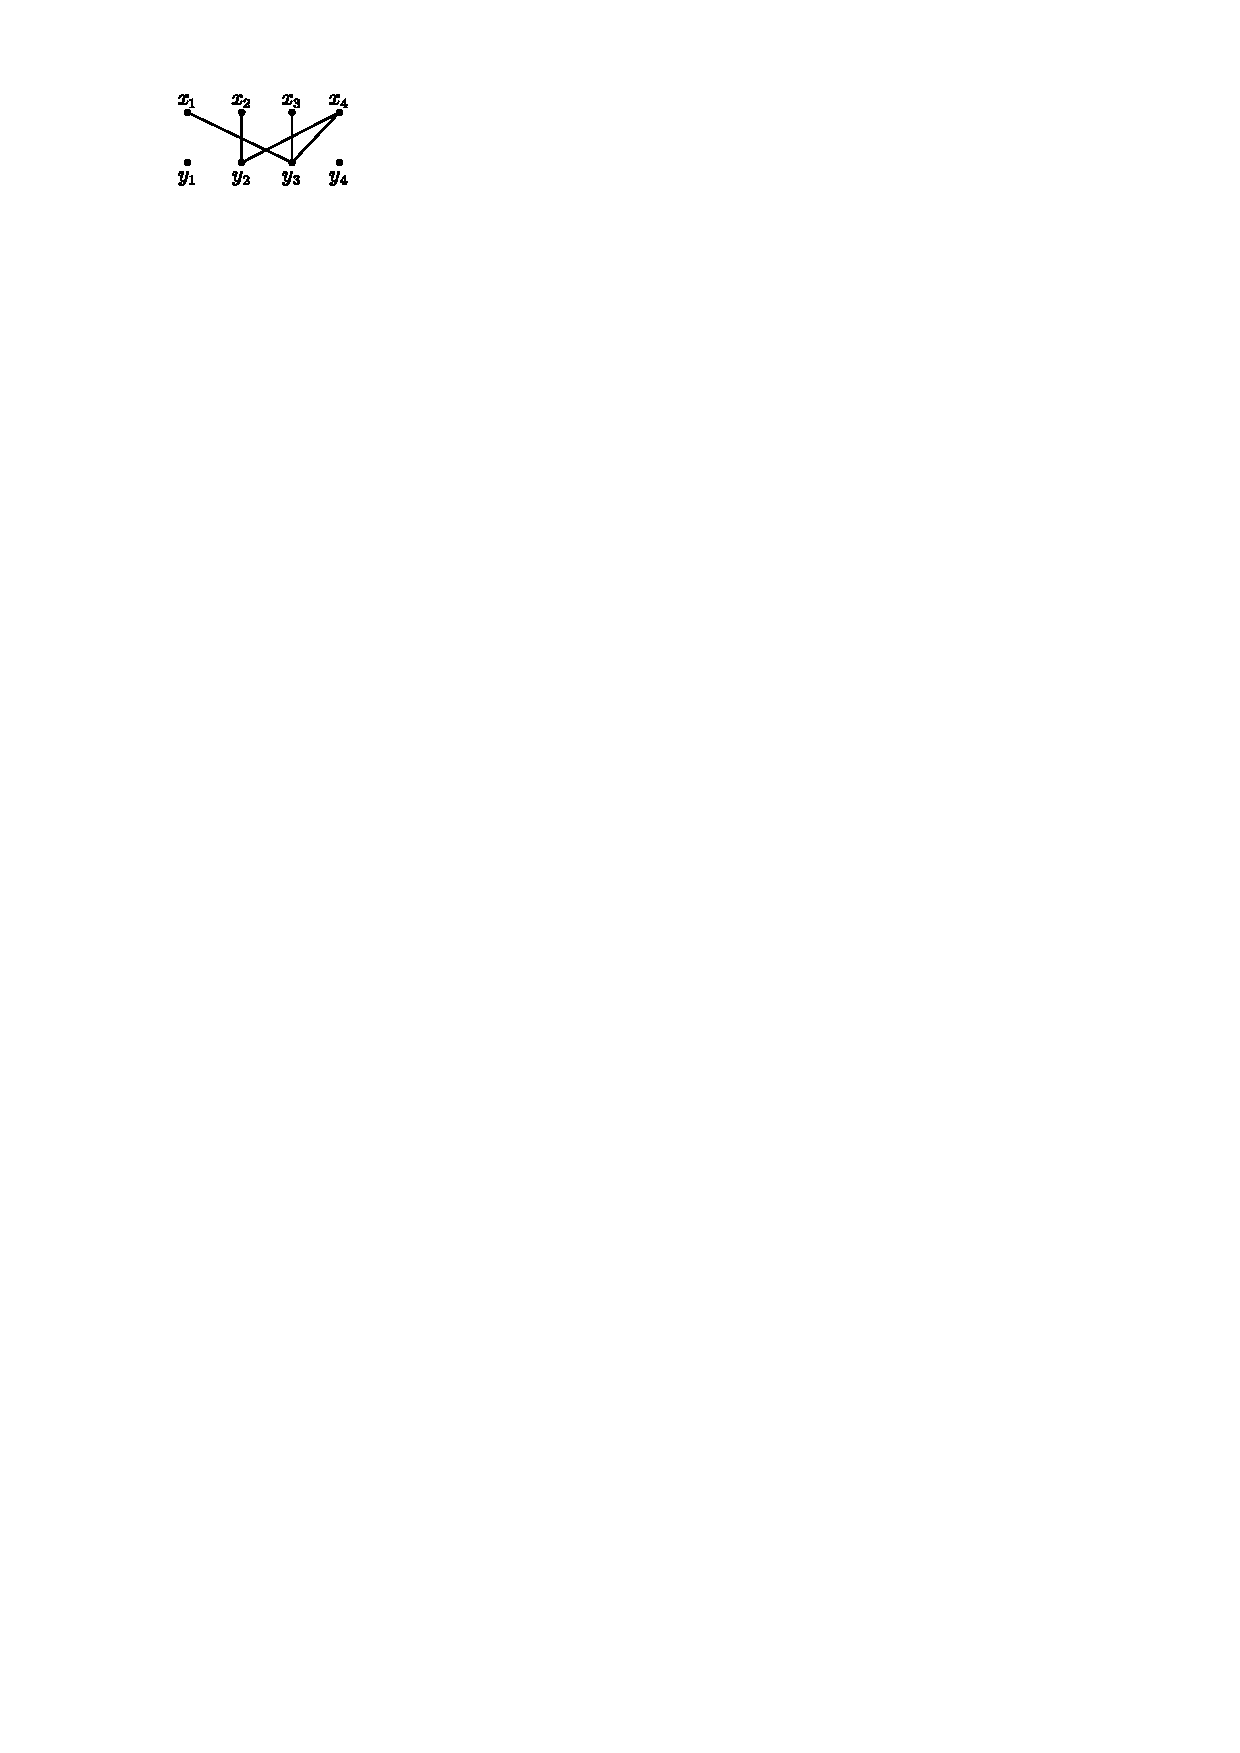
\includegraphics[scale=1.2]{image/CH5_zuiyoupipei1.pdf}  
		%\caption{信息包结构} 
		\label{fikgkjjjl1KKk}  
	\end{figure}

{\noindent}	 \rule[0pt]{\textwidth}{0.05em}
在$G_l$中选一个匹配$M=\{x_2y_2,x_3y_3\}$,$M$不饱和,$x_4$为$M$非饱和点,置$S=\{x_4\}, T=\phi$

$N_{G_l}(S)=\{y_2,y_3\}\supset T$, 选择$y_2\in N_{G_l}(S)-T=\{y_2,y_3\}$,$y_2$是$M$的饱和点,且$y_2x_2\in M$. 置$S=S\cup \{x_2\}=\{x_4,x_2\}, T=T\cup\{y_2\}=\{y_2\}$;

$N_{G_l}(S)=\{y_2,y_3\}\supset T$, 选择$y_3\in N_{G_l}(S)-T=\{y_3\}$,$y_3$是$M$的饱和点,且$y_3x_3\in M$. 置$S=S\cup \{x_3\}=\{x_2, x_3,x_4\}, T=T\cup\{y_3\}=\{y_2, y_3\}$;

$N_{G_l}(S)=\{y_2,y_3\}= T$,求得$\alpha_l=1$.

\noindent(2) 根据$\alpha_l=1$更新可行顶点标号$\hat{l}$为:
	\[
\begin{blockarray}{ccccc}
	\begin{block}{(cccc)c}
		12&14&15&14&15\\
		9&11&6&8&10\\
		10&9&16&14&15\\
		12&13&13&10&12\\
	\end{block}
	0&1&1&0&
\end{blockarray}
\]
关于$\hat{l}$的相等子图$G_{\hat{l}}$,如下:
\begin{figure}[H]
	\small
	\centering 
	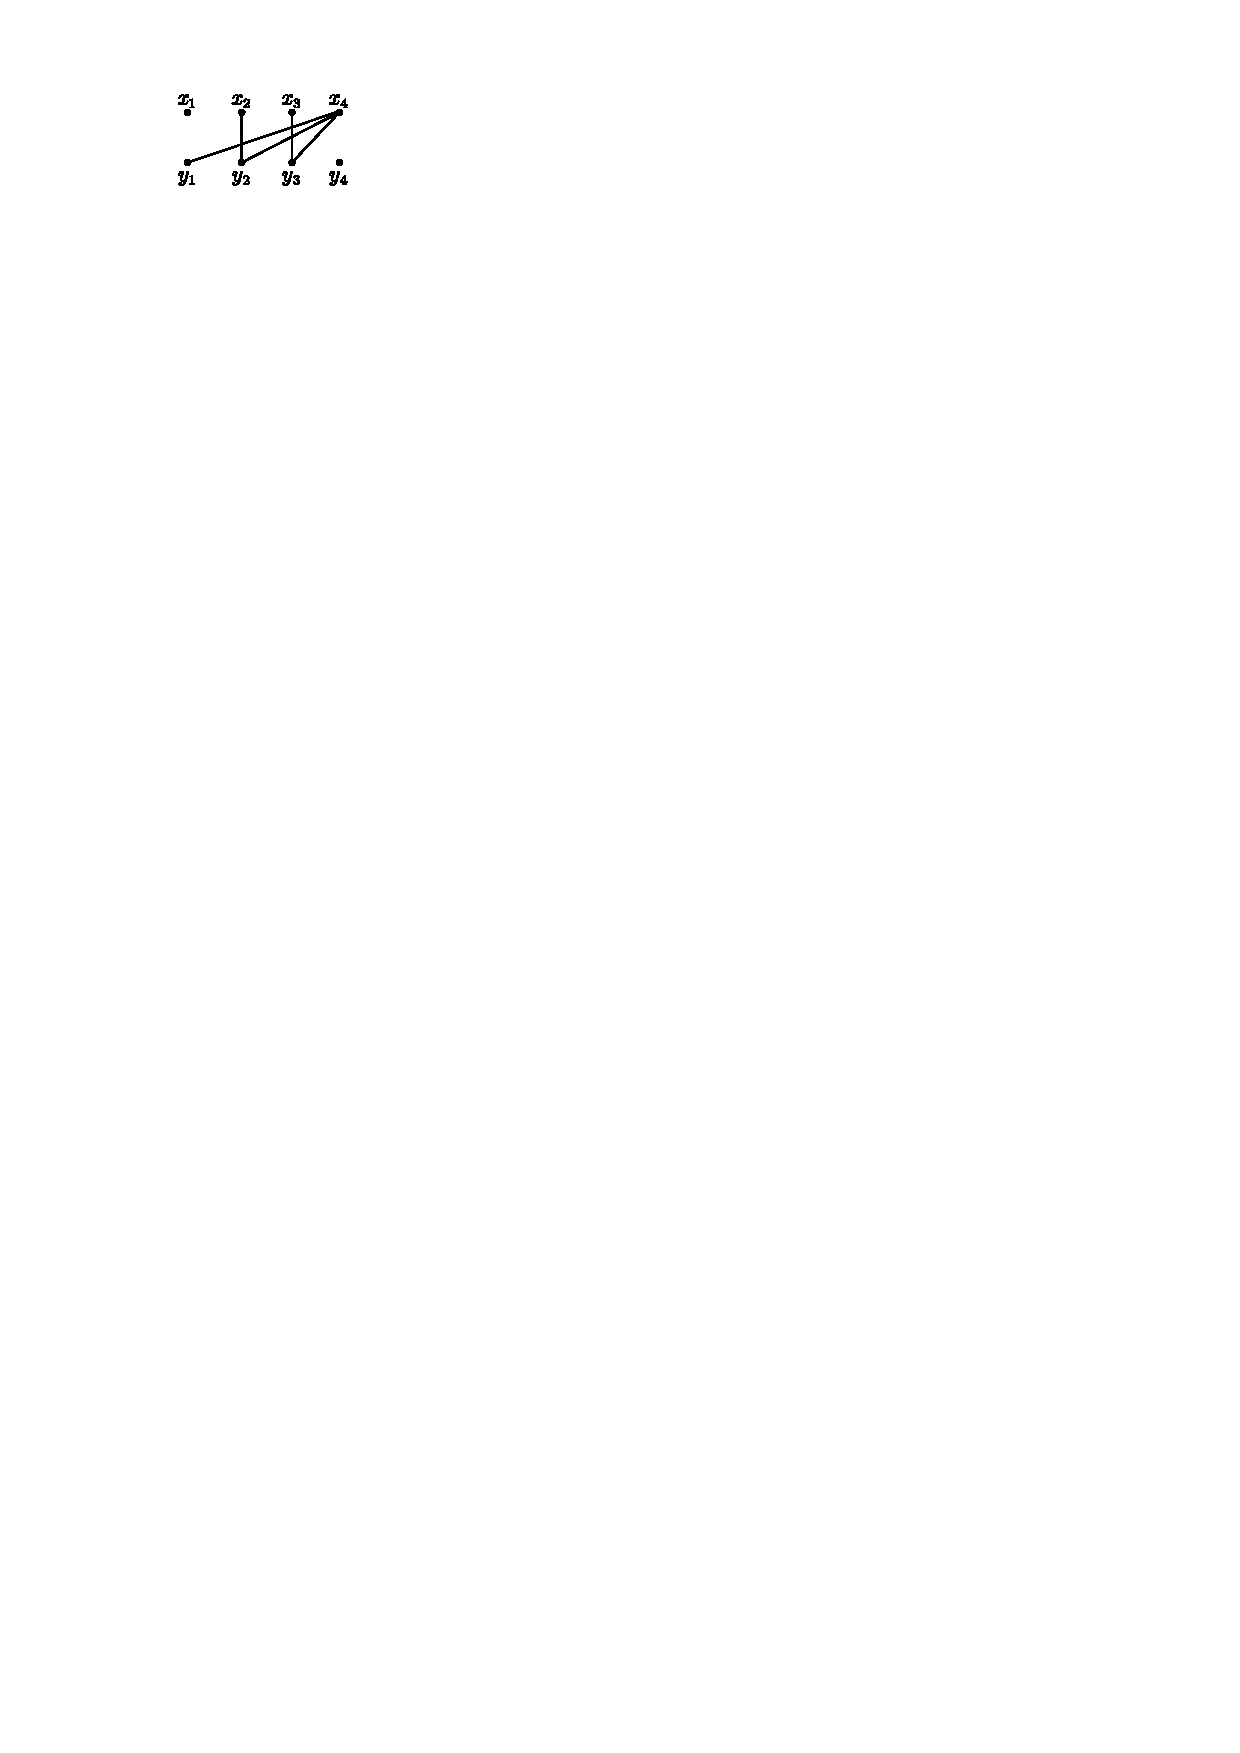
\includegraphics[scale=1.2]{image/CH5_zuiyoupipei2.pdf}  
	%\caption{信息包结构} 
	\label{fikgksjjjl1KKk}  
\end{figure}




在$G_l$中选一个匹配$M=\{x_2y_2,x_3y_3,x_4y_1\}$,$M$不饱和,$x_1$为$M$非饱和点,置$S=\{x_1\}, T=\phi$

$N_{G_{\hat{l}}}(S)=T=\phi$.

{\noindent}\textcolor{red}{\heiti {标准答案没有这一部分}}

{\noindent}	 \rule[0pt]{\textwidth}{0.05em}


\noindent(3) 寻找$S, T$使得$N(S)=T$. 此时$S=\{x_1,x_2,x_3,x_4\}, T=\{y_2, y_3\}$,求得$\alpha=1$.

根据$\alpha_{l^{'}}=1$更新可行顶点标号$l^{'}$为:
	\[
\begin{blockarray}{ccccc}
	\begin{block}{(cccc)c}
		12&14&15&14&14\\
		9&11&6&8&10\\
		10&9&16&14&15\\
		12&13&13&10&12\\
	\end{block}
	0&1&1&0&
\end{blockarray}
\]

关于${l^{'}}$的相等子图$G_{l^{'}}$,如下:
\begin{figure}[H]
	\small
	\centering 
	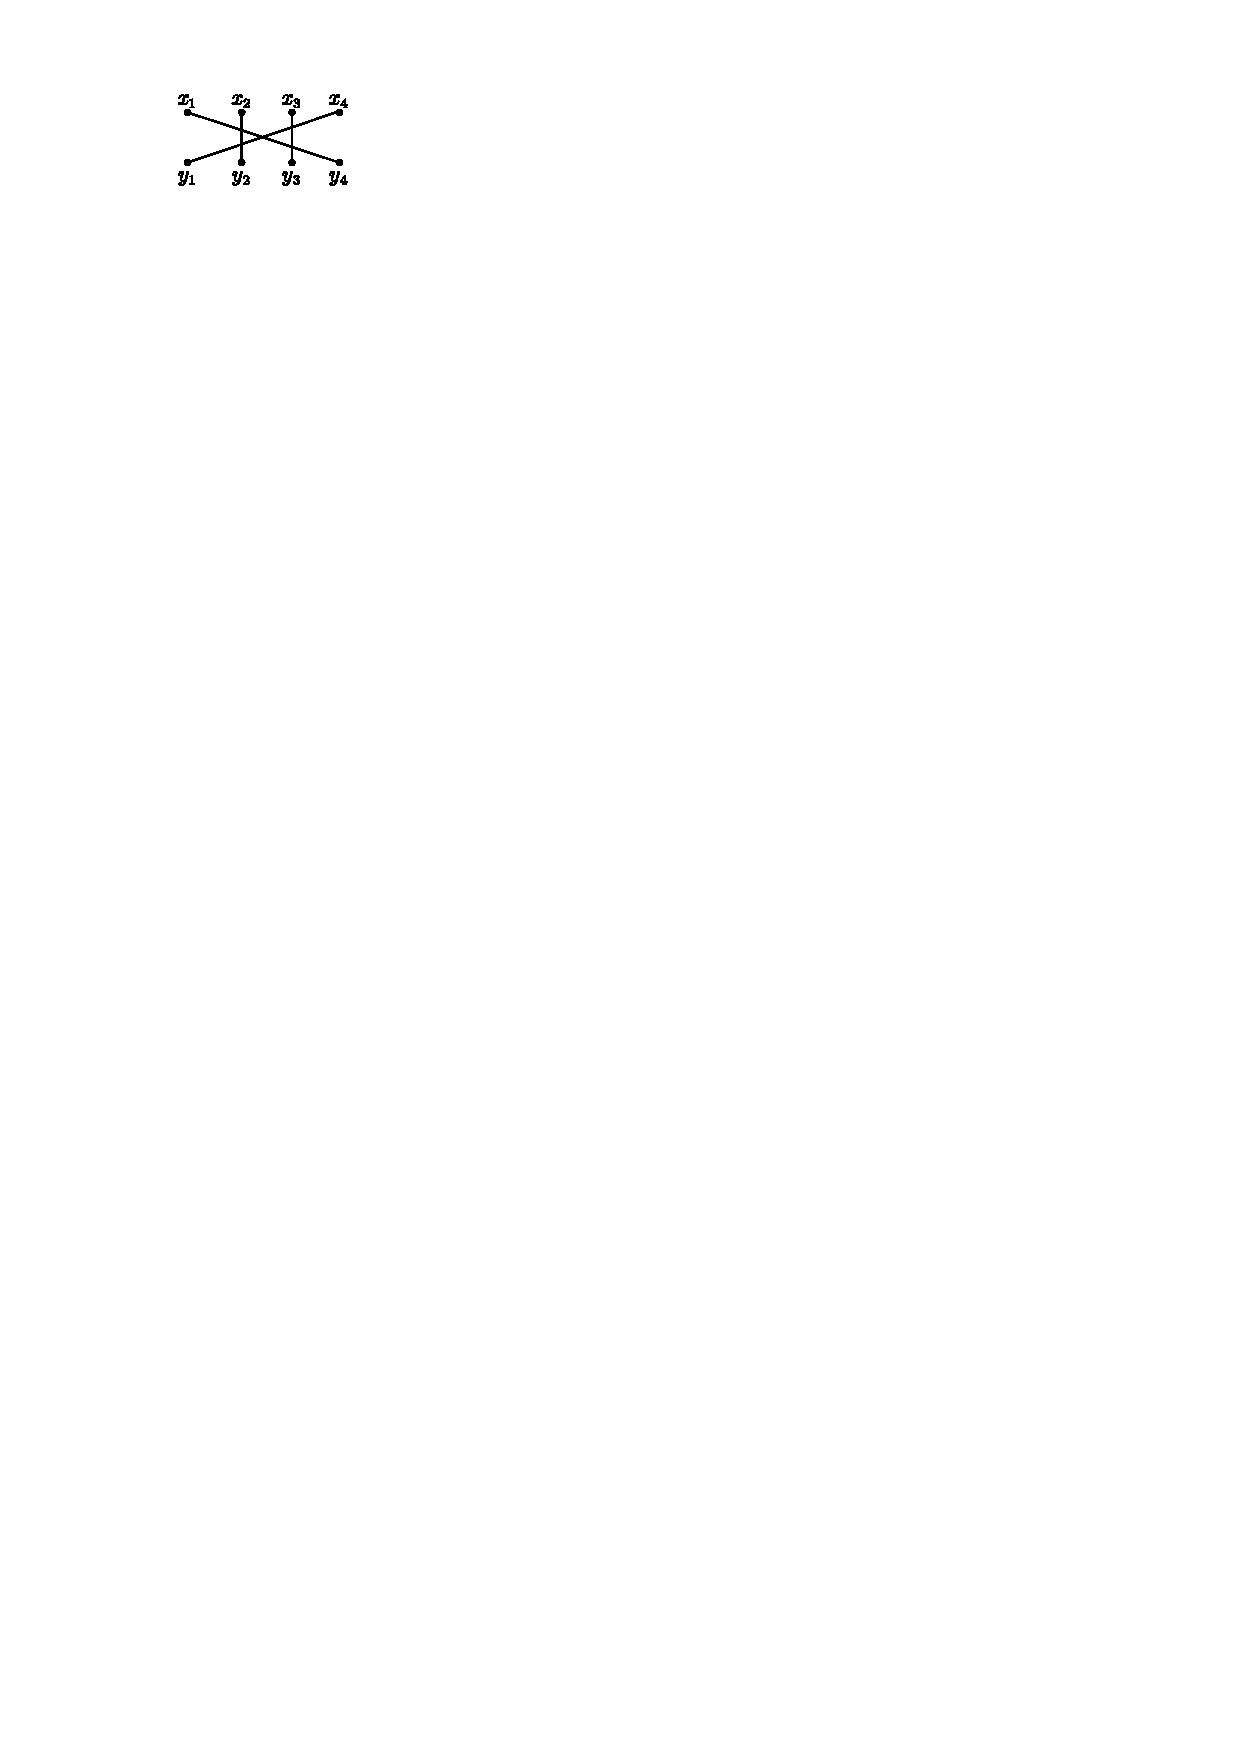
\includegraphics[scale=1.2]{image/CH5_zuiyoupipei3.pdf}  
	%\caption{信包结构} 
	\label{fikgksjjl1KKk}  
\end{figure}

得到最优匹配:$\{x_1y_4,x_2y_2,x_3y_3, x_4y_1\}$,即第1个工人分配第4份工作,第2个工人分配第2份工作,第3个工人分配第3份工作,第4个工人分配第1份工作.





\end{example}









